\documentclass{standalone}
\usepackage{tikz}
\usetikzlibrary{
  arrows,
  calc,
  decorations.pathmorphing,
  decorations.pathreplacing,
  decorations.markings,
  fadings,
  positioning,
  shapes,
  arrows.meta
}
\pgfdeclareradialshading{glow}{\pgfpoint{0cm}{0cm}}{
  color(0mm)=(white);
  color(5mm)=(white);
  color(9mm)=(black);
  color(10mm)=(black)
}

\begin{tikzfadingfrompicture}[name=glow fading]
  \shade [shading=glow] (0,0) circle (1);
\end{tikzfadingfrompicture}

\ifpdf
% Ensure reproducible output
\pdfinfoomitdate=1
\pdfsuppressptexinfo=-1
\pdftrailerid{}
\fi

\begin{document}

\begin{tikzpicture}[scale=1.5391]
  \node at (0, 0) {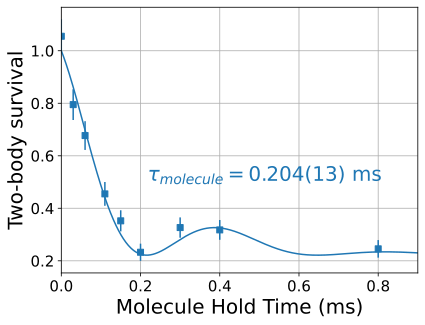
\includegraphics[width=7.6958cm]{imgs/exp_data_norm_m_t.pdf}};
  \node at (-2.35, 1.7) {\footnotesize (\textbf{a})};
  \node at (0, -3.9) {\includegraphics[width=7.6958cm]{imgs/exp_data_norm_a_t.pdf}};
  \node at (-2.35, 1.5 - 3.9) {\footnotesize (\textbf{b})};
  % strength = 2pi 29.3(17) mHz/mW^2.58
  \node at (0.85, -3.25) {\includegraphics[width=4.6175cm]{imgs/atomic_loss_scaling_inset.pdf}};
\end{tikzpicture}

\end{document}
